\documentclass[a4paper]{article} 
\input{head}
\begin{document}

%Title section

\fancyhead[C]{}
\hrule \medskip % Upper rule
\begin{minipage}{0.295\textwidth} 
\raggedright
\footnotesize
Chaitanya Kapoor \hfill\\   
2020A3PS1219P\hfill\\
f20201219@pilani.bits-pilani.ac.in
\end{minipage}
\begin{minipage}{0.4\textwidth} 
\centering 
\Large
Maths F111 Formulae
\end{minipage}
\begin{minipage}{0.295\textwidth} 
\raggedleft
\today\hfill\\
\end{minipage}
\medskip\hrule 
\bigskip
Miscellaneous coordinate systems:
\begin{itemize}
    \item Polar coordinates: \[\begin{cases}
                                 x=r\cos{\theta}\\
                                 y=r\sin{\theta}
                            \end{cases}\]
    \item Cylindrical coordinates: $r\geq 0, 0\leq \theta \leq 2\pi, -\infty < z < \infty$
                            \[\begin{cases}
                                 x=r\cos{\theta}\\
                                 y=r\sin{\theta}\\
                                 z=z 
                            \end{cases}\]
    \item Spherical coordinates: $\rho$ = Distance from origin, $\phi$ = Angle with \textbf{positive} $z-$axis, $\theta$ = Angle with $x$ axis
                            \[\begin{cases}
                                 x=\rho\sin{\phi}\cos{\theta}\\
                                 y=\rho\sin{\phi}\sin{\theta}\\
                                 z=\rho\cos{\phi}
                            \end{cases}\]
\end{itemize}
\section{Vector valued functions}
\begin{itemize}
\item Parametric equation of a line passing through $(x_0,y_0,z_0)$ and parallel to $a\hat{i}+b\hat{j}+c\hat{k}$:
                            \[\begin{cases}
                                 x(t) = x_0+ta\\
                                 y(t) = y_0+tb\\
                                 z(t) = z_0+tc
                            \end{cases}\]
\item Arc length of a curve for $a\leq x\leq b$:
    \begin{equation*}
        L = \int_{a}^{b}\sqrt{\left(\frac{dx}{dt}\right)^2+\left(\frac{dy}{dt}\right)^2+\left(\frac{dz}{dt}\right)^2}dt
    \end{equation*}
    Arc length parameter $\vec{s}(t)$ = $\int_{t_0}^{t}|v(\tau)|d\tau$
\item Unit tangent vector $\vec{T}(t)=\frac{\vec{v}(t)}{|\vec{v}(t)|}=\frac{d\vec{r}}{d\vec{s}}$, $\vec{s}$ being the arc length parameter
\item Curvature $(\kappa)$:
        \begin{equation*}
            \kappa = \left|{\frac{d\overrightarrow{T}}{ds}}\right| = \left|{\frac{d\overrightarrow{T}/dt}{ds/dt}}\right| = \frac{1}{|\vec{v}|}\left|{\frac{d\overrightarrow{T}}{dt}}\right|
        \end{equation*}
    Unit normal $(\overrightarrow{N})$: 
        \begin{equation*}
            \overrightarrow{N} = \frac{\left(\frac{d\overrightarrow{T}}{ds}\right)}{\left|\frac{d\overrightarrow{T}}{ds}\right|} = \frac{1}{\kappa}\left(\frac{d\overrightarrow{T}}{ds}\right)
        \end{equation*}
Curvature can also be written in terms of $v$ and $a$ as $\frac{|\vec{v}\times\vec{a}|}{|\vec{v}|^3}$
\item $\vec{a}(t) = \frac{d|v|}{dt}\overrightarrow{T}+\kappa|\vec{v}|^2\overrightarrow{N}$
\item Binormal vector $(\overrightarrow{B}) = \overrightarrow{T}\times\overrightarrow{N}$ \\
$\overrightarrow{T}$ and $\overrightarrow{N}$: Osculating plane\\
$\overrightarrow{B}$ and $\overrightarrow{N}$: Normal plane\\
$\overrightarrow{B}$ and $\overrightarrow{T}$: Rectifying plane
\item Torsion $\tau$ = $-\frac{d\overrightarrow{B}}{ds}\cdot\overrightarrow{N}$
\end{itemize}
\newpage

\section{Polar coordinates}
\begin{itemize}
\item Important polar curves:
\begin{enumerate}
    \item $r = 1-\cos{\theta}$, $r = 1+\cos{\theta}$:\\
        \begin{center}
        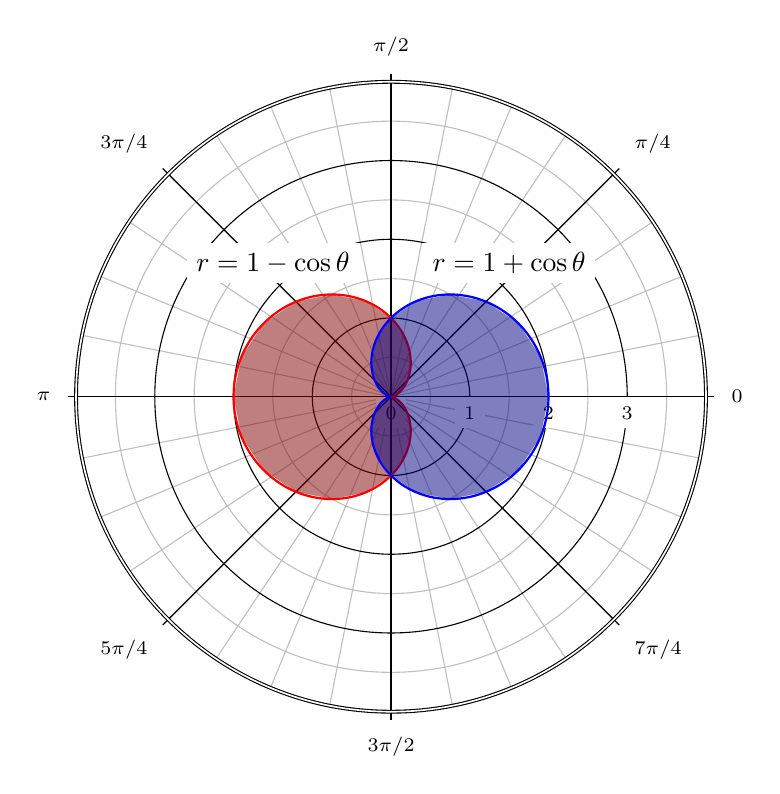
\begin{tikzpicture}[]
            % Draw the lines at multiples of pi/12
            \foreach \ang in {0,...,31} {
              \draw [lightgray] (0,0) -- (\ang * 180 / 16:4);
            }
            % Concentric circles and radius labels
            \foreach \s in {0, 1, 2, 3} {
              \draw [lightgray] (0,0) circle (\s + 0.5);
              \draw (0,0) circle (\s);
              \node [fill=white] at (\s, 0) [below] {\scriptsize $\s$};
            }
            % Add the labels at multiples of pi/4
            \foreach \ang/\lab/\dir in {
              0/0/right,
              1/{\pi/4}/{above right},
              2/{\pi/2}/above,
              3/{3\pi/4}/{above left},
              4/{\pi}/left,
              5/{5\pi/4}/{below left},
              7/{7\pi/4}/{below right},
              6/{3\pi/2}/below} {
              \draw (0,0) -- (\ang * 180 / 4:4.1);
              \node [fill=white] at (\ang * 180 / 4:4.2) [\dir] {\scriptsize $\lab$};
            }
            
            % The double-lined circle around the whole diagram
            \draw [style=double] (0,0) circle (4);
            
            \fill [fill=red!50!black, opacity=0.5] plot [domain=0:2*pi]
              (xy polar cs:angle=\x r, radius= {1-cos(\x r)});
            \draw [thick, color=red, domain=0:2*pi, samples=200, smooth]
              plot (xy polar cs:angle=\x r, radius={1-cos(\x r)});
            \node [fill=white] at (-1.5,1.7) {$r=1-\cos\theta$};
            \fill [fill=blue!50!black, opacity=0.5] plot [domain=0:2*pi]
              (xy polar cs:angle=\x r, radius= {1+cos(\x r)});
            \draw [thick, color=blue, domain=0:2*pi, samples=200, smooth]
              plot (xy polar cs:angle=\x r, radius={1+cos(\x r)});
            \node [fill=white] at (1.5,1.7) {$r=1+\cos\theta$};
        \end{tikzpicture}
        \end{center}
    \item $r = 1+\sin{\theta}, r = 1-\sin{\theta}$:\\
        \begin{center}
        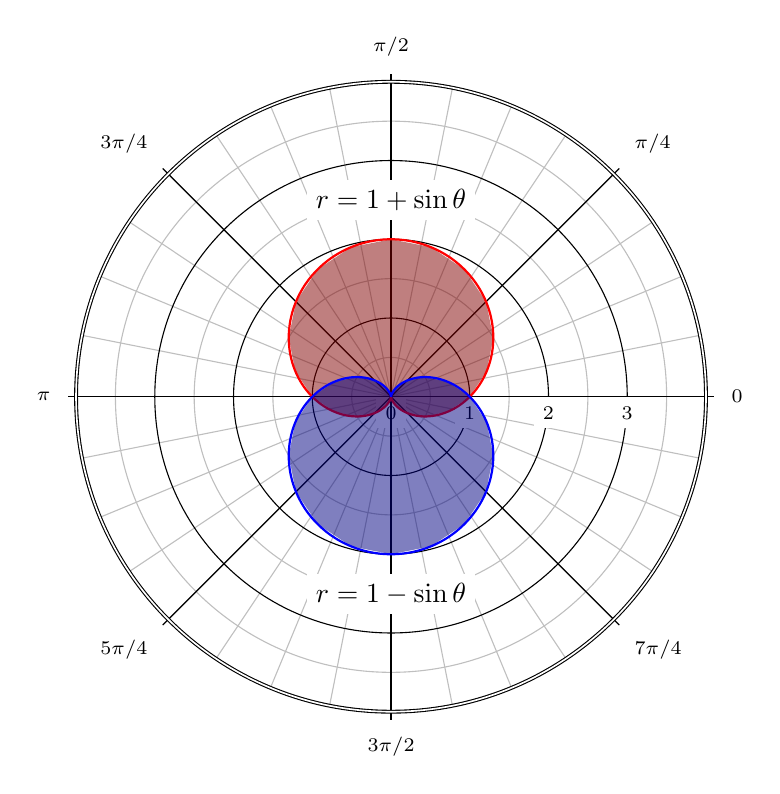
\begin{tikzpicture}[]
            % Draw the lines at multiples of pi/12
            \foreach \ang in {0,...,31} {
              \draw [lightgray] (0,0) -- (\ang * 180 / 16:4);
            }
            % Concentric circles and radius labels
            \foreach \s in {0, 1, 2, 3} {
              \draw [lightgray] (0,0) circle (\s + 0.5);
              \draw (0,0) circle (\s);
              \node [fill=white] at (\s, 0) [below] {\scriptsize $\s$};
            }
            % Add the labels at multiples of pi/4
            \foreach \ang/\lab/\dir in {
              0/0/right,
              1/{\pi/4}/{above right},
              2/{\pi/2}/above,
              3/{3\pi/4}/{above left},
              4/{\pi}/left,
              5/{5\pi/4}/{below left},
              7/{7\pi/4}/{below right},
              6/{3\pi/2}/below} {
              \draw (0,0) -- (\ang * 180 / 4:4.1);
              \node [fill=white] at (\ang * 180 / 4:4.2) [\dir] {\scriptsize $\lab$};
            }
            
            % The double-lined circle around the whole diagram
            \draw [style=double] (0,0) circle (4);
            
            \fill [fill=red!50!black, opacity=0.5] plot [domain=0:2*pi]
              (xy polar cs:angle=\x r, radius= {1+sin(\x r)});
            \draw [thick, color=red, domain=0:2*pi, samples=200, smooth]
              plot (xy polar cs:angle=\x r, radius={1+sin(\x r)});
            \node [fill=white] at (0,2.5) {$r=1+\sin\theta$};
            \fill [fill=blue!50!black, opacity=0.5] plot [domain=0:2*pi]
              (xy polar cs:angle=\x r, radius= {1-sin(\x r)});
            \draw [thick, color=blue, domain=0:2*pi, samples=200, smooth]
              plot (xy polar cs:angle=\x r, radius={1-sin(\x r)});
            \node [fill=white] at (0,-2.5) {$r=1-\sin\theta$};
        \end{tikzpicture}
        \end{center}
    \newpage
    \item $r = |\sin{\theta}|$:\\
        \begin{center}
            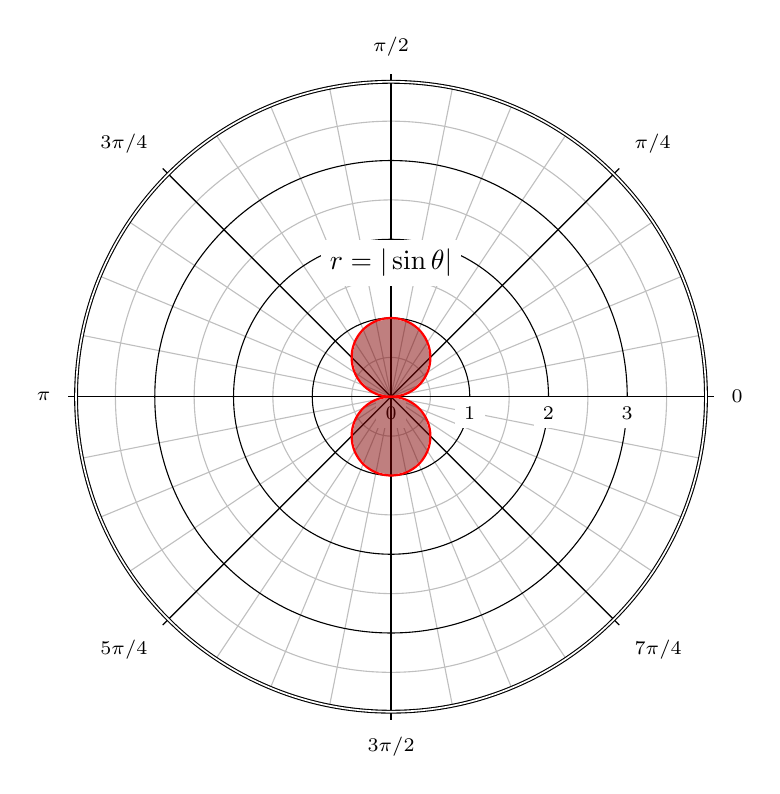
\begin{tikzpicture}[]
            % Draw the lines at multiples of pi/12
            \foreach \ang in {0,...,31} {
              \draw [lightgray] (0,0) -- (\ang * 180 / 16:4);
            }
            % Concentric circles and radius labels
            \foreach \s in {0, 1, 2, 3} {
              \draw [lightgray] (0,0) circle (\s + 0.5);
              \draw (0,0) circle (\s);
              \node [fill=white] at (\s, 0) [below] {\scriptsize $\s$};
            }
            % Add the labels at multiples of pi/4
            \foreach \ang/\lab/\dir in {
              0/0/right,
              1/{\pi/4}/{above right},
              2/{\pi/2}/above,
              3/{3\pi/4}/{above left},
              4/{\pi}/left,
              5/{5\pi/4}/{below left},
              7/{7\pi/4}/{below right},
              6/{3\pi/2}/below} {
              \draw (0,0) -- (\ang * 180 / 4:4.1);
              \node [fill=white] at (\ang * 180 / 4:4.2) [\dir] {\scriptsize $\lab$};
            }
            
            % The double-lined circle around the whole diagram
            \draw [style=double] (0,0) circle (4);
            
            \fill [fill=red!50!black, opacity=0.5] plot [domain=0:2*pi]
              (xy polar cs:angle=\x r, radius= {sin(\x r)});
            \draw [thick, color=red, domain=0:2*pi, samples=200, smooth]
              plot (xy polar cs:angle=\x r, radius={sin(\x r)});
            \node [fill=white] at (0,1.7) {$r=|\sin{\theta}|$};
            \fill [fill=red!50!black, opacity=0.5] plot [domain=0:2*pi]
              (xy polar cs:angle=\x r, radius= {-sin(\x r)});
            \draw [thick, color=red, domain=0:2*pi, samples=200, smooth]
              plot (xy polar cs:angle=\x r, radius={-sin(\x r)});
        \end{tikzpicture}
        \end{center}
    \item $r = \sin{2\theta}$:\\
            \begin{center}
            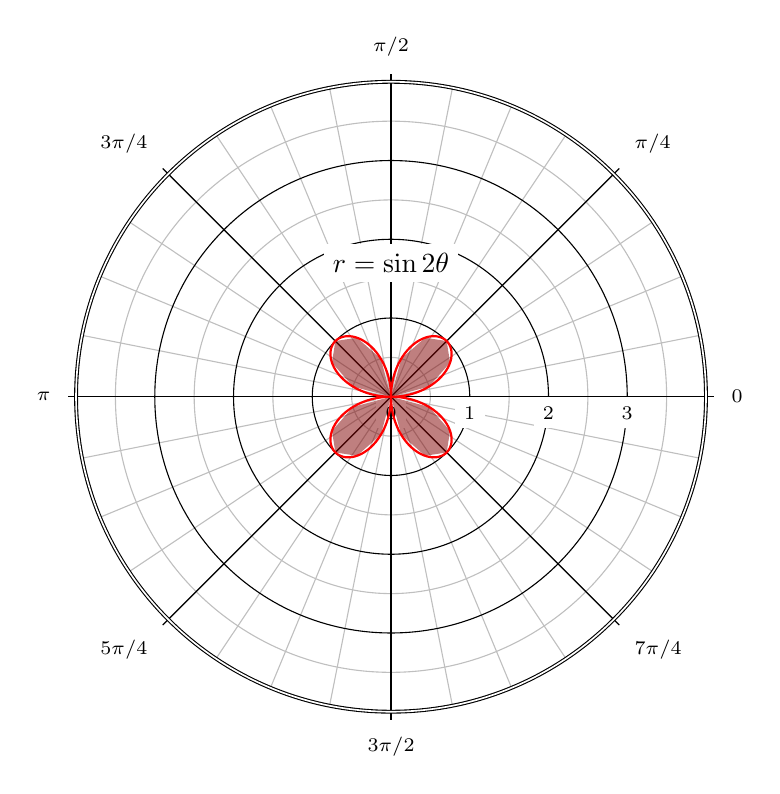
\begin{tikzpicture}[]
            % Draw the lines at multiples of pi/12
            \foreach \ang in {0,...,31} {
              \draw [lightgray] (0,0) -- (\ang * 180 / 16:4);
            }
            % Concentric circles and radius labels
            \foreach \s in {0, 1, 2, 3} {
              \draw [lightgray] (0,0) circle (\s + 0.5);
              \draw (0,0) circle (\s);
              \node [fill=white] at (\s, 0) [below] {\scriptsize $\s$};
            }
            % Add the labels at multiples of pi/4
            \foreach \ang/\lab/\dir in {
              0/0/right,
              1/{\pi/4}/{above right},
              2/{\pi/2}/above,
              3/{3\pi/4}/{above left},
              4/{\pi}/left,
              5/{5\pi/4}/{below left},
              7/{7\pi/4}/{below right},
              6/{3\pi/2}/below} {
              \draw (0,0) -- (\ang * 180 / 4:4.1);
              \node [fill=white] at (\ang * 180 / 4:4.2) [\dir] {\scriptsize $\lab$};
            }
            
            % The double-lined circle around the whole diagram
            \draw [style=double] (0,0) circle (4);
            
            \fill [fill=red!50!black, opacity=0.5] plot [domain=0:2*pi]
              (xy polar cs:angle=\x r, radius= {sin(2*\x r)});
            \draw [thick, color=red, domain=0:2*pi, samples=200, smooth]
              plot (xy polar cs:angle=\x r, radius={sin(2*\x r)});
            \node [fill=white] at (0,1.7) {$r=\sin{2\theta}$};
        \end{tikzpicture}
        \end{center}
    \newpage
    \item $r = 1+\sin{2\theta}$:\\
                    \begin{center}
            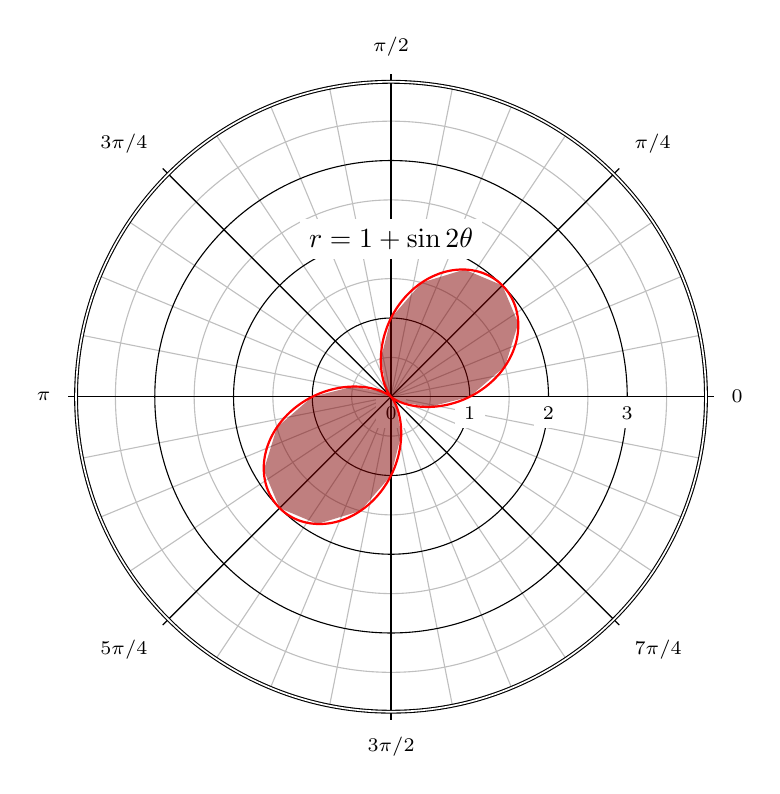
\begin{tikzpicture}[]
            % Draw the lines at multiples of pi/12
            \foreach \ang in {0,...,31} {
              \draw [lightgray] (0,0) -- (\ang * 180 / 16:4);
            }
            % Concentric circles and radius labels
            \foreach \s in {0, 1, 2, 3} {
              \draw [lightgray] (0,0) circle (\s + 0.5);
              \draw (0,0) circle (\s);
              \node [fill=white] at (\s, 0) [below] {\scriptsize $\s$};
            }
            % Add the labels at multiples of pi/4
            \foreach \ang/\lab/\dir in {
              0/0/right,
              1/{\pi/4}/{above right},
              2/{\pi/2}/above,
              3/{3\pi/4}/{above left},
              4/{\pi}/left,
              5/{5\pi/4}/{below left},
              7/{7\pi/4}/{below right},
              6/{3\pi/2}/below} {
              \draw (0,0) -- (\ang * 180 / 4:4.1);
              \node [fill=white] at (\ang * 180 / 4:4.2) [\dir] {\scriptsize $\lab$};
            }
            
            % The double-lined circle around the whole diagram
            \draw [style=double] (0,0) circle (4);
            
            \fill [fill=red!50!black, opacity=0.5] plot [domain=0:2*pi]
              (xy polar cs:angle=\x r, radius= {1+sin(2*\x r)});
            \draw [thick, color=red, domain=0:2*pi, samples=200, smooth]
              plot (xy polar cs:angle=\x r, radius={1+sin(2*\x r)});
            \node [fill=white] at (0,2) {$r=1+\sin{2\theta}$};
        \end{tikzpicture}
        \end{center}
\end{enumerate}
\item Area enclosed by a polar curve:
    \begin{equation*}
        A = \frac{1}{2} \int_{\alpha}^{\beta}r^2d\theta
    \end{equation*}
    Length of a polar curve:
    \begin{equation*}
        L = \int_{\alpha}^{\beta}\sqrt{r^2+\left(\frac{dr}{d\theta}\right)^2}d\theta
    \end{equation*}
\end{itemize}

\section{Partial derivatives}
\begin{itemize}
    \item From the $1^{st}$ principles, the partial derivative of a function $f(x,y)$ with respect to $x$ is given as:
    \begin{equation*}
        \frac{\partial f}{\partial x} = f_x = \lim_{\Delta x \to 0} \frac{f(x+\Delta x,y)-f(x,y)}{\Delta x}
    \end{equation*}
    A similar idea is followed for  calculating $\frac{\partial f}{\partial y}$
    
    \item Implicit differentiation: Let $f(x,y) = c$. After a bit of work, we get the following
    \begin{equation*}
        \frac{dy}{dx} = -\frac{f_x}{f_y} 
    \end{equation*}
    
    \item Higher order partial derivatives:
    \begin{align*}
        \frac{\partial^2 f}{\partial x^2} &= f_{xx} = \lim_{h \to 0} \frac{f_x(x+h,y)-f_x(x,y)}{h}\\
        \frac{\partial^2 f}{\partial y\partial x} &= f_{xy} = \lim_{k\to 0} \frac{f_x(x,y+k)-f_x(x,y)}{k}
    \end{align*}
    
    \item Directional derivative : $\left(\frac{df}{dt}\right)_{\hat{n}} = \nabla f\cdot\hat{n}$
    \item Angle between $2$ surfaces : $\theta = \cos^{-1}{\left(\frac{\nabla f\cdot\nabla g}{|\nabla f||\nabla g|}\right)}$
    \item Equation of tangent plane at $(x_0,y_0,z_0)$: $(x-x_0)f_x+(y-y_0)f_y+(z-z_0)f_z=0$\\
    Equation of normal at $(x_0,y_0,z_0)$:
    \begin{equation*}
        \frac{x-x_0}{f_x} = \frac{y-y_0}{f_y} = \frac{z-z_0}{f_z}
    \end{equation*}
    
    \item Linearization of $f(x,y)$ at $(x_0,y_0)$:\\
    \begin{equation*}
        f(x,y) \approx f(x_0,y_0) + (x-x_0)f_x(x_0,y_0)+(y-y_0)f_y(x_0,y_0)
    \end{equation*}
    \item Extrema: At the critical points: $f_x(x_0,y_0) = 0; f_y(x_0,y_0) = 0$\\
    If at $(x_0,y_0)$:
    \begin{enumerate}
        \item $f_{xx}f_{yy}-f_{xy}^2 > 0; f_{xx}<0 \implies$ \textbf{Local max} \item $f_{xx}f_{yy}-f_{xy}^2 > 0; f_{xx}>0 \implies$ \textbf{Local min}
        \item $f_{xx}f_{yy}-f_{xy}^2 < 0 \implies$ \textbf{Saddle point}
        \item $f_{xx}f_{yy}-f_{xy}^2 = 0 \implies$ \textbf{Further investigation}
    \end{enumerate}
    
    \item Lagrange multipliers: For a function $f(x,y,z)$ subject to the constraints $g_1(x,y,z)$ and $g_2(x,y,z)$, we have:
    \begin{equation*}
        \nabla f = \lambda\nabla g_1 + \mu\nabla g_2
    \end{equation*}
\end{itemize}

\section{Multiple integrals}
\begin{itemize}
    \item Double integrals to compute volume over a region $R$ under a surface $f(x,y)$:
    \begin{equation*}
        V = \iint\limits_Rf(x,y)dA
    \end{equation*}
    For computing the area of a closed bounded region $R$:
    \begin{equation*}
        A = \iint\limits_RdA
    \end{equation*}
    Average value of $f$ over a region $R$ = $\displaystyle\frac{1}{\text{Area of R}}\iint\limits_R fdA$
    
    \item Volume in polar coordinates:
    \begin{equation*}
        V = \iint\limits_R f(r,\theta)rdrd\theta
    \end{equation*}
    
    \item Triple integrals in cylindrical coordinates:
    \begin{equation*}
        I = \iiint\limits_R f(r,\theta,z)dV = \iiint\limits_R f(r,\theta,z)dzrdrd\theta
    \end{equation*}
    Triple integrals in spherical coordinates:
    \begin{equation*}
        I = \iiint\limits_R f(\rho,\phi,\theta)dV = \iiint\limits_R f(\rho,\phi,\theta)\rho^2\sin{\phi}d\rho d\phi d\theta 
    \end{equation*}
    
    \item Substitutions in iterated integrals:
    \begin{enumerate}
        \item Double integrals: For a coordinate transformation $x=g(u,v)$ and $y=h(u,v)$, we define the \textbf{Jacobian} as $J(u,v)=\frac{\partial(x,y)}{\partial(u,v)}$:
        \begin{equation*}
        J(u,v)=
            \begin{vmatrix}
            \frac{\partial x}{\partial u} & \frac{\partial x}{\partial v}\\
            \frac{\partial y}{\partial u} & \frac{\partial y}{\partial v}
        \end{vmatrix} 
        \end{equation*}
        The new integral becomes:
        \begin{equation*}
            \iint\limits_Rf(x,y)dxdy = \iint\limits_Rf(g(u,v),h(u,v))\left|\frac{\partial(x,y)}{\partial(u,v)}\right|dudv
        \end{equation*}
        
        \item Triple integrals: Following a similar set of steps as above, we introduce a new transformation for the $z$ coordinate as $z=k(u,v,w)$. The Jacobian changes to a $3\times3$ determinant in this case to give the new integral:
        \begin{equation*}
            \iiint\limits_Df(x,y,z)dxdydx = \iiint\limits_G h(u,v,w)|J(u,v,w)|dudvdw
        \end{equation*}
        Where $h(u,v,w)$ is the transform of $f(x,y,z)$
    \end{enumerate}
\end{itemize}

\section{Integrals and vector fields}
\begin{itemize}
    \item Line integral of $f$ over a curve $C$:
    \begin{equation*}
        \int_{C} f(x,y,z)ds = \int_{a}^{b}f(x(t),y(t),z(t))|\vec{v}(t)|dt
    \end{equation*}
    Line integral over a vector field $\overrightarrow{F}$: $\int_{c}\overrightarrow{F\cdot} d\vec{r}$
    \item Work done by a force $\overrightarrow{F}(x,y,z)$ over a smooth curve $C$ with the parametrization $\vec{r}(t)$:
    \begin{equation*}
        W = \int_{C}\overrightarrow{F}\cdot\overrightarrow{T}ds
    \end{equation*}
    \item Flux of a vector field $F = M(x,y)\hat{i}+N(x,y)\hat{j}$ with the \textbf{outward normal} $\vec{n} = \overrightarrow{T}\times\vec{k}$:
    \begin{equation*}
        \int_{C}\overrightarrow{F}\cdot\vec{n}dx = \int_{C}(My'(t)-Nx'(t))dt
    \end{equation*}
    
    \item Circulation of a vector field $F = M(x,y,z)\hat{i}+N(x,y,z)\hat{j}+P(x,y,z)\hat{k}$:
    \begin{equation*}
        \oint_{C}\overrightarrow{F}\cdot d\vec{r} = \oint Mdx+Ndy+Pdz = \int_{C}(Mx'(t)+Ny'(t)+Pz'(t))dt
    \end{equation*}
    \item If $\overrightarrow{F}$ is conservative $\Leftrightarrow \overrightarrow{F} = \nabla f$\\
    $\oint_{C}\overrightarrow{F}\cdot d\vec{r} = 0$ over every closed curve if $\overrightarrow{F}$ is a conservative field
    \item If $\overrightarrow{F}$ is conservative, then $\text{curl}(\overrightarrow{F}) = 0$, which is given as:
    \begin{equation*}
        \text{curl}(F) = \nabla\times\overrightarrow{F} = 
        \begin{vmatrix}
            \hat{i} & \hat{j} & \hat{k}\\
            \frac{\partial}{\partial x} & \frac{\partial}{\partial y} & \frac{\partial}{\partial z}\\
            M & N & P
        \end{vmatrix} = 0
    \end{equation*}
    
    \item Green's theorem: 
    \begin{enumerate}
        \item Circulation-curl/tangential form:
        \begin{equation*}
            \oint_{C}\overrightarrow{F}\cdot\overrightarrow{T}ds = \oint_{C}Mdx+Ndy = \iint\limits_R\left(\frac{\partial N}{\partial x}-\frac{\partial M}{\partial y}\right)dxdy
        \end{equation*}
        \item Flux-divergence/normal form:
        \begin{equation*}
             \oint_{C}\overrightarrow{F}\cdot\hat{n}ds = \oint_{C}Mdx-Ndy = \iint\limits_R\left(\frac{\partial M}{\partial x}+\frac{\partial N}{\partial y}\right)dxdy
        \end{equation*}
    \end{enumerate}
    \item Surface area of $f(x,y,z)=c$ over a region $R$ with the unit normal vector $\vec{p}$ is given as:
        \begin{equation*}
            A = \iint\limits_Sd\sigma = \iint\limits_R\frac{|\nabla f|}{|\nabla f\cdot\vec{p}|}dA
        \end{equation*}
    For a surface of the form $f(x,y,z) = z-m(x,y)$ with the projeted region $R$ in the $XY$ plane:
    \begin{equation*}
        A = \iint\limits_Sd\sigma = \iint\limits_R\sqrt{1+m_x^2+m_y^2}dA
    \end{equation*}
    
    \item A surface $\vec{r}(t)$ parametrized as $\vec{r}(u,v)$ has the surface area $A$ = $\iint\limits_Sd\sigma=\iint\limits_R|\vec{r_u}\times\vec{r_v}|dudv$
    
    \item Surface integral of $g(x,y,z)$ over the projected region $S$ of the function $f(x,y,z)=c$ is:
    \begin{equation*}
        \iint\limits_R g(x,y,z)\frac{|\nabla f|}{|\nabla f\cdot\vec{p}|}dA
    \end{equation*}
    Similarly, the surface integral of a vector field $F$ over a surface $S$ is
    $\iint\limits_C\overrightarrow{F}\cdot\hat{n}d\sigma$ and the flux over the region is $\pm\iint\limits_R\frac{F\cdot\nabla f}{|\nabla f\cdot p|}dA$. The sign of flux depends on \textbf{the choice of the normal vector}
    
    \item Stoke's theorem:
        \begin{equation*}
            \oint_{C}\overrightarrow{F}\cdot d\vec{r} = \iint\limits_S(\nabla\times\overrightarrow{F})\cdot\hat{n}d\sigma = \iint\limits_S\left(\frac{\partial N}{\partial x}-\frac{\partial M}{\partial y}\right)dxdy
        \end{equation*}
        This integral can be taken over a region $R$ to give:
        \begin{equation*}
             \oint_{C}\overrightarrow{F}\cdot d\vec{r} = \iint\limits_R\frac{(\nabla\times\overrightarrow{F})\cdot\nabla f}{|\nabla f\cdot\hat{p}|}dA
        \end{equation*}
        For a surface parametrized as $r(u,v)$, the integral takes the form:
        \begin{equation*}
             \oint_{C}\overrightarrow{F}\cdot d\vec{r} = \iint\limits_R(\nabla\times\overrightarrow{F})\cdot(\vec{r_u}\times\vec{r_v})dudv
        \end{equation*}
    
    \item Divergence theorem: The divergence of a vector field $F=M\hat{i}+N\hat{j}+P\hat{k}$ is given as:
    \begin{equation*}
        \text{div}(\overrightarrow{F}) = \nabla\cdot\overrightarrow{F} = \frac{\partial M}{\partial x}+\frac{\partial N}{\partial y}+\frac{\partial P}{\partial z} 
    \end{equation*}
    The flux of a vector fielf $\overrightarrow{F}$ over a surface $S$ in the direction of the outward normal $\hat{n}$ is calculated by the integral:
    \begin{equation*}
        \iint\limits_S\overrightarrow{F}\cdot\hat{n}d\sigma = \iiint\limits_D(\nabla\cdot\overrightarrow{F})dV
    \end{equation*}
\end{itemize}

\section{Infinite series}
For the sake of brevity, I define two series: $\sum a_n=a_n$ and $\sum b_n=b_n$
\begin{itemize}
    \item Integral test: If $f(x)$ is $+ve$, continuous and decreasing $\forall x\geq N$ for some $N$, then $a_n$ and $\int_{N}^{\infty}f(x)dx$ converge or diverge together

    \item $p-$series: $\sum \frac{1}{n^p}$ is \textbf{convergent} for $p>1$ and \textbf{divergent} for $p\leq 1$ 
    \item Direct comparison test:
        \begin{enumerate}
            \item If $a_n\leq b_n \forall n\geq N$ and $b_n$ is convergent, then $a_n$ is also convergent
            \item If $a_n\geq b_n \forall n\geq N$ and $b_n$ is divergent, then $a_n$ is also divergent
        \end{enumerate}
        
    \item Limit comparison test: $a_n,b_n$ are $+ve$ $\forall n\geq N$, then:
    \begin{enumerate}
        \item $\displaystyle\lim_{n\to\infty}\left(\frac{a_n}{b_n}\right)=c$ which is \textit{finite and nonzero}, then $a_n$ and $b_n$ \textbf{converge or diverge together}
        \item  $\displaystyle\lim_{n\to\infty}\left(\frac{a_n}{b_n}\right)=0$ , and if $b_n$ \textbf{converges} then $a_n$ \textbf{converges}
        \item $\displaystyle\lim_{n\to\infty}\left(\frac{a_n}{b_n}\right)=\infty$, and if $b_n$ \textbf{diverges} then $a_n$ \textbf{diverges}
    \end{enumerate}
    
    \item Ratio test: If $\displaystyle\lim_{n\to\infty}\left(\frac{a_{n+1}}{a_n}\right)=r$, then:
    \begin{enumerate}
        \item $r<1 \implies a_n$ is \textbf{convergent}
        \item $r>1 \implies a_n$ is \textbf{divergent}
        \item $r=1 \implies$ \textbf{inconclusive}
    \end{enumerate}
    
    \item Root test: If $\displaystyle\lim_{n\to\infty}\left(a_n\right)^{1/n}=r$, then:
    \begin{enumerate}
        \item $r<1 \implies a_n$ is \textbf{convergent}
        \item $r>1 \implies a_n$ is \textbf{divergent}
        \item $r=1 \implies$ \textbf{inconclusive}
    \end{enumerate}
    
    \item Lebinitz's test: An alternating series $\sum(-1)^{n+1}u_{n}$ converges if:
    \begin{enumerate}
        \item $u_n\geq u_{n+1}\forall n\geq N$ for some $N$
        \item $\displaystyle\lim_{n\to\infty}u_n=0$
    \end{enumerate}
    
    \item Radius of convergence $R$ of a power series $\sum a_n(x-a)^n$ is given by the relation:
    \begin{equation*}
        \frac{1}{R}=\lim_{n\to\infty}\left|\frac{a_{n+1}}{a_n}\right| = \lim_{n\to\infty}|a_n|^{1/n}
    \end{equation*}
    
    \item Taylor series for a function $f(x)$ about the point $x=a$ is given by:
    \begin{equation*}
        \sum_{n=0}^{\infty}\frac{f^n(a)}{n!}(x-a)^n = f(a)+\frac{f'(a)}{1!}(x-a)+\frac{f''(a)}{2!}(x-a)^2+\dots
    \end{equation*}
    The \textbf{Maclaurin series} are the Taylor series generated at $a=0$
\end{itemize}
\end{document}
